\documentclass[../main.tex]{subfiles} 
\usepackage{ctex}
\usepackage{xltxtra}
\usepackage{graphicx}
\usepackage{booktabs}
\usepackage{amsmath}
\usepackage{mathdots}
\usepackage{amssymb}
\usepackage{cite}
\usepackage{appendix}
\usepackage{array}
\usepackage{subfigure}
\usepackage{makecell}
\begin{document}

    \subsection{数据总体分布浏览}

        首先,利用head()函数,可以查看数据集中前五条数据,结合题目中的数据说明对数据集进行了解,如图1所示。

        \begin{figure}[H]
            \centering
            \includegraphics[scale=0.5]{sec2_1.png}
            \caption{数据展示}
            \label{tu2_1}
        \end{figure}

        在表1中,对于每个属性我做了一个详细解释:
        
        其中PassengerId的形式为gggg\_pp,gggg指的是乘客所在的团体,pp是乘客在团体中的编号。通常一个团体中的成员都是一个家庭。
        Cabin的形式为Deck/Number/Side。Deck指的是桌子编号,Number指的是乘客在桌子中的编号,Side指的是桌子所在位置。
        具体的每个属性取值会在后续进行解释。
            
        \begin{table}[H] 
            \centering
            \begin{tabular}{|c|c|} 
                \hline 
                \textbf{Feature} & \textbf{Explanation} \\ \hline 
                PassengerId & 每个乘客的唯一标志 \\ \hline 
                HomePlanet & 乘客出发的星球 \\ \hline 
                CryoSleep & 乘客是否进入休眠状态 \\ \hline 
                Cabin & 乘客居住的舱室 \\ \hline 
                Destination & 乘客到达的星球 \\ \hline 
                Age & 乘客的年龄 \\ \hline 
                VIP & 乘客是否在航行过程中为VIP服务付费 \\ \hline
                RoomService & 乘客在房间服务上的消费数目\\ \hline
                FoodCourt & 乘客在餐厅中的消费数目\\ \hline
                ShoppingMall & 乘客在超市中的消费数目\\ \hline
                Spa & 乘客在水疗按摩服务中的消费数目\\ \hline
                VRDeck & 乘客在VR游戏中的消费数目\\ \hline 
                Name & 乘客的姓氏与名字 \\ \hline 
                Transported & 乘客是否被传送到另一个维度 \\ \hline 
            \end{tabular} 
            \caption{数据集属性解释}
        \end{table}

        接下来我对于数据集的相关信息进行了一个查看,如图2所示。可以看到的是,训练集中有8693条数据,14列特征,其中Transported是数据集的标签;测试集有4277条数据,13列特征,缺少了数据集的标签。
        首先我们可以看到数据的类型主要有三种:\textbf{PassengerId、HomePlanet、CryoSleep、Cabin、Destination、VIP、Name都为obeject型数据;
        Age、RoomService、FoodCourt、ShoppingMall、Spa、VRDeck都为float64型数据;标签Transported是bool型数据}。
        其次可以发现训练集和测试集缺失现象非常严重,训练集中只有乘客的唯一表征PassengerId和标签Transported不存在缺失,而测试集中甚至只有PassengerId不存在缺失。
        因此后续想要有一个好的预测结果,必须要对于数据进行一个较好的补充。

        \begin{figure}[ht]
            \centering
            \subfigure[训练集数据摘要]
            {
                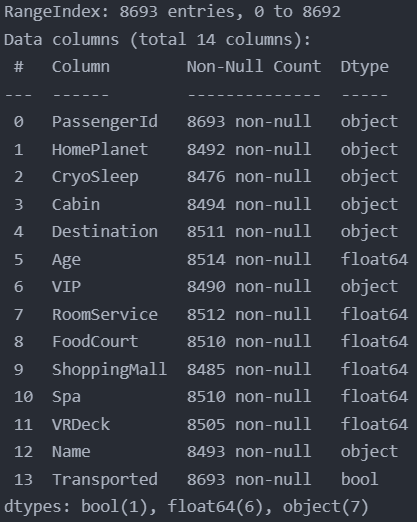
\includegraphics[scale=0.6]{Sec2_2.png}
            }
            \subfigure[测试集数据摘要]
            {
                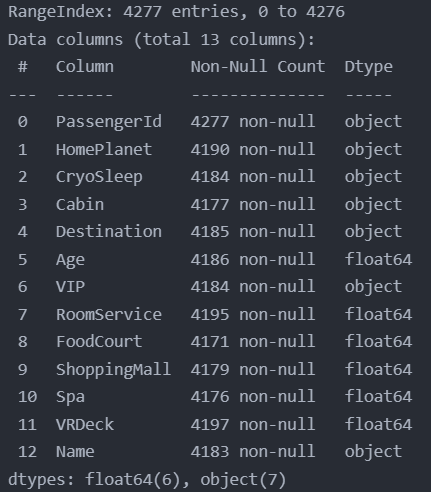
\includegraphics[scale=0.6]{Sec2_3.png}
            }
            \label{tu2_2}
            \caption{数据集摘要}
        \end{figure}

        最后,我查看了数值型数据的分布情况,如图3所示。可以发现的是六个数值型数据的均值和标准差较大,后续应该要在数据归一化的过程中对于年龄进行分组处理,而对于其他五个费用数据应该要通过对数变换减小数据的偏差,便于模型学习。

        \begin{figure}[ht]
            \centering
            \subfigure[训练集数值型数据分布]
            {
                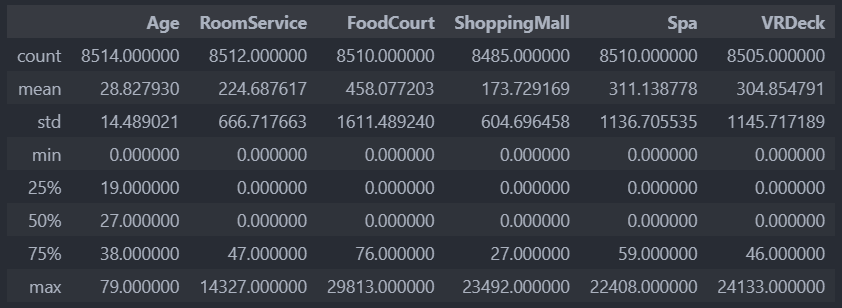
\includegraphics[scale=0.6]{Sec2_4.png}
            }
            \subfigure[测试集数值型数据分布]
            {
                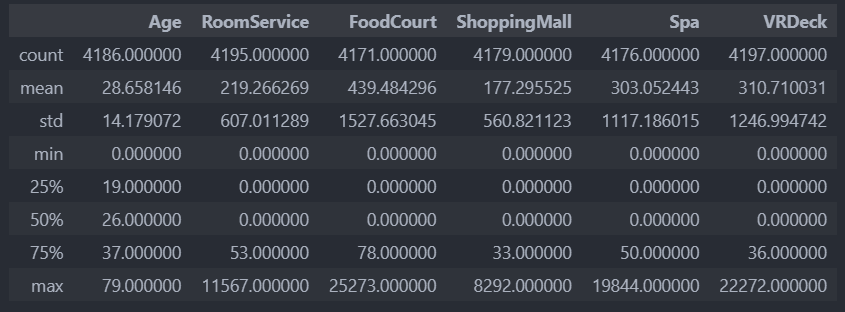
\includegraphics[scale=0.6]{Sec2_5.png}
            }
            \label{tu2_3}
            \caption{数据集数值型数据分布}
        \end{figure}

    \subsection{数据特征可视化}

        首先查看训练集中标签Transported的分布情况,如图4所示。可以发现正如背景中所说,被传送者和不被传送者大概是1:1的分布,这也加大了传送原因的分析难度,需要后续结合多种特征进行分析。

        \begin{figure}[H]
            \centering
            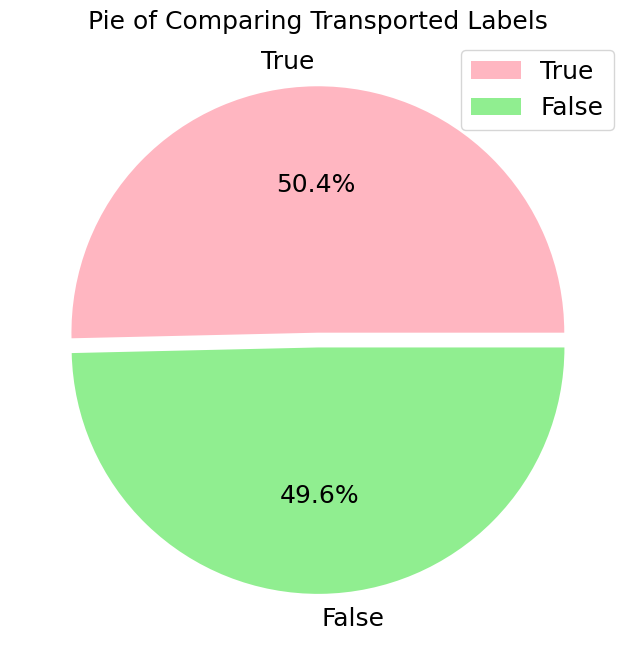
\includegraphics[scale=0.4]{Sec2_6.png}
            \label{tu2_4}
            \caption{标签Transported分布}
        \end{figure}

        其次查看休眠人数的对比及是否休眠与是否被传送的关系,如图5所示。
        可以发现的是休眠的人数大约有不休眠的人数的60\%,而休眠的人中有大约80\%被传送,而不休眠的人中只有大约30\%被传送。
        可以发现休眠状态下更有可能被传送,因此可以认为休眠是一个重要的特征,与标签Transported有较强的相关性。

        \begin{figure}[H]
            \centering
            \subfigure[休眠人数对比]
            {
                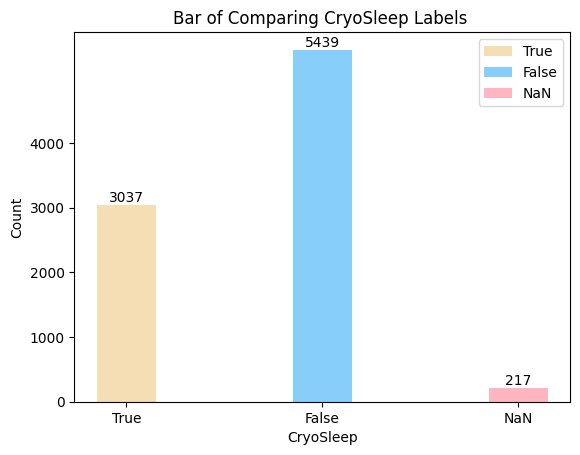
\includegraphics[scale=0.5]{Sec2_7.png}
            }
            \subfigure[是否休眠与是否被传送]
            {
                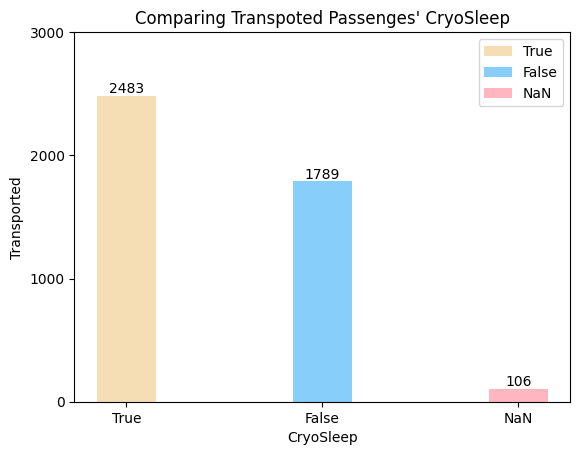
\includegraphics[scale=0.5]{Sec2_8.png}
            }
            \label{tu2_5}
            \caption{CryoSleep}
        \end{figure}

        查看VIP人数的对比与VIP和Transported之间的关系,如图6所示。
        可以发现不是VIP的乘客占比非常高,达到了95.4\%,而是VIP的乘客和缺失值的乘客人数相近。
        并且可以发现,不是VIP的乘客中被传送的比例比是VIP的乘客被传送的比例高了大约12\%。
        但是由于不是VIP的乘客人数远远高于是VIP的乘客人数,因此我觉得VIP与Transported并没有非常强的相关性。

        \begin{figure}[H]
            \centering
            \subfigure[VIP人数对比]
            {
                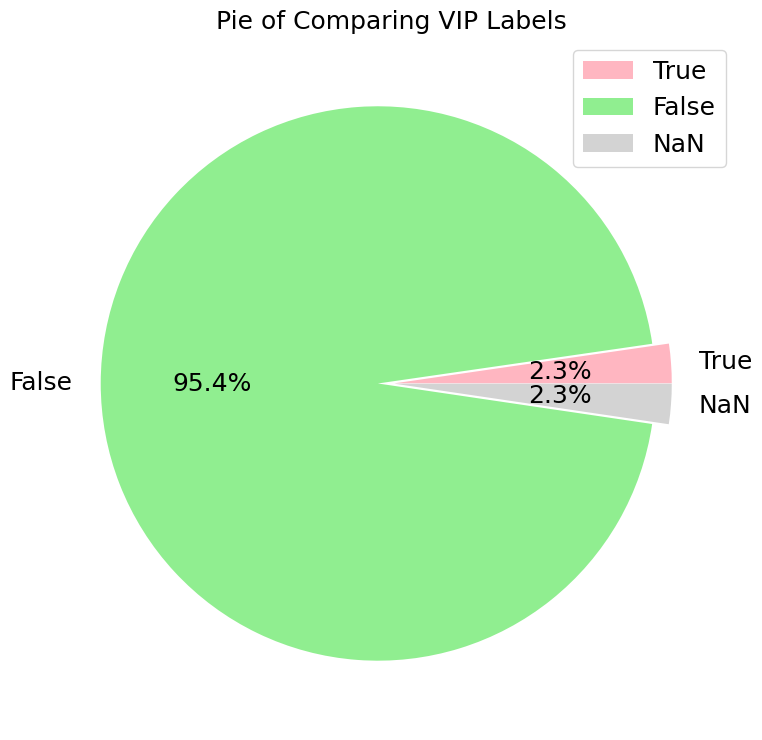
\includegraphics[scale=0.4]{Sec2_9.png}
            }
            \subfigure[VIP与Transported]
            {
                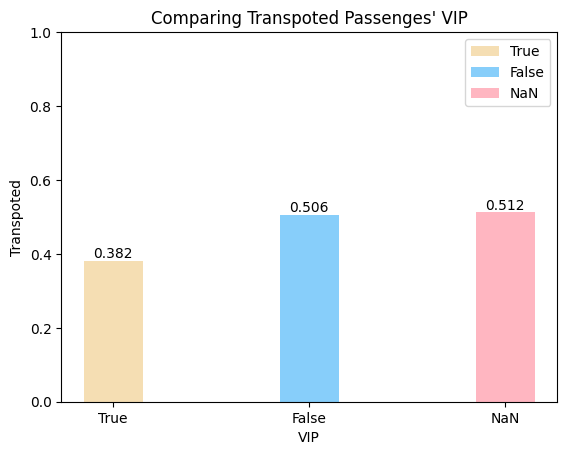
\includegraphics[scale=0.5]{Sec2_10.png}
            }
            \label{tu2_6}
            \caption{VIP}
        \end{figure}

        查看HomePlanet与Transported之间的关系,如图7所示。
        HomePlanet有三种取值,分别是Europa、Earth、Mars和缺失值,其中来自Earth的人数最多。
        但是可以发现,来自Earth的乘客被传送走的比例反而是最少的,而来自Europa的乘客被传送走的比例反而是最高的,相差达到了23\%。
        因此可以认为HomePlanet也是一个较为重要的特征值。

        \begin{figure}[H]
            \centering
            \subfigure[HomePlanet对比]
            {
                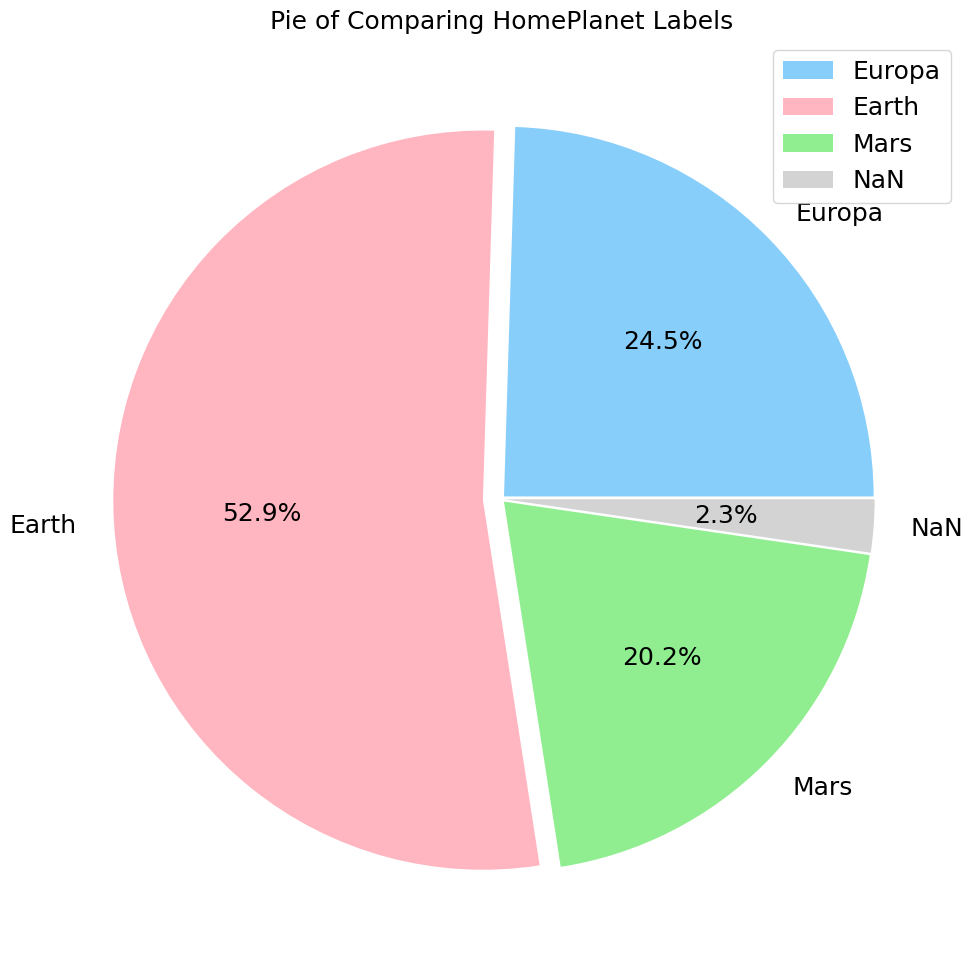
\includegraphics[scale=0.3]{Sec2_11.png}
            }
            \subfigure[HomePlanet与Transported]
            {
                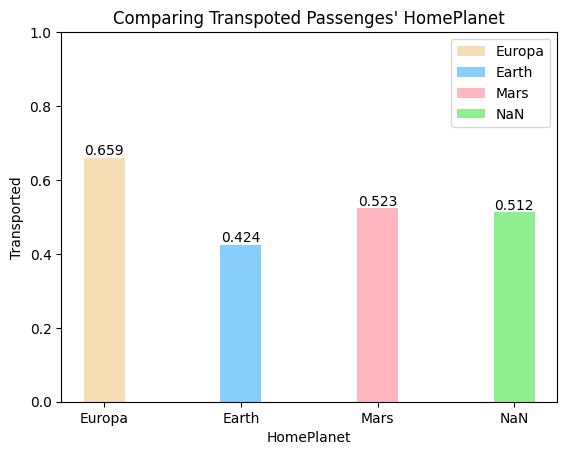
\includegraphics[scale=0.5]{Sec2_12.png}
            }
            \label{tu2_7}
            \caption{HomePlanet}
        \end{figure}

        查看Destination与Transported之间的关系,如图8所示。
        同样的,Destination有三种取值,分别是TRAPPIST-1e、PSO J318.5-22、55 Cancri e和缺失值,其中前往TRAPPIST-1e的人数最多,占比达到68\%。
        但是同样可以发现,前往TRAPPIST-1e的乘客被传送走的比例反而是最少的,而前往55 Cancri e的乘客被传送走的比例反而是最高的,相差达到了14\%。
        不过两者之间的差别并没有HomePlanet之中那么大,因此认为Destination特征对于是否被传送的影响小于HomePlanet特征。

        \begin{figure}[H]
            \centering
            \subfigure[Destination对比]
            {
                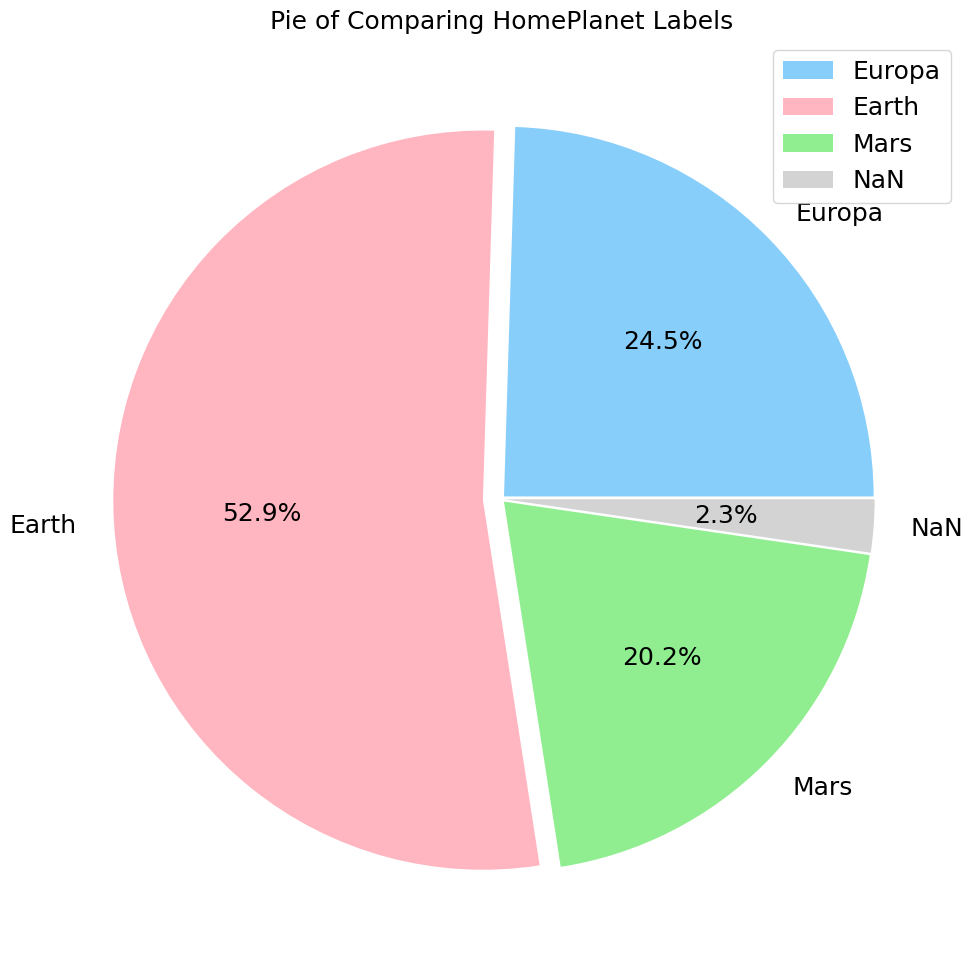
\includegraphics[scale=0.3]{Sec2_13.png}
            }
            \subfigure[Destination与Transported]
            {
                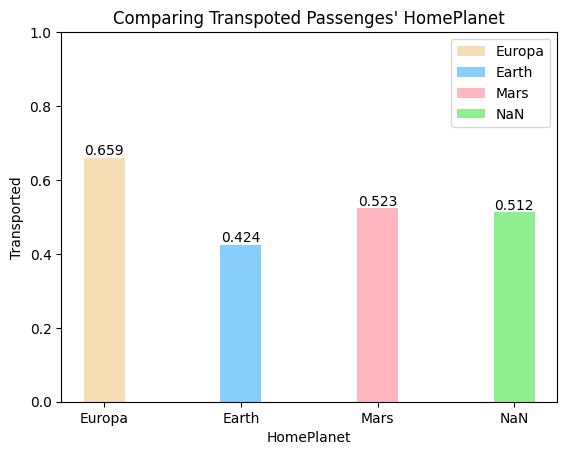
\includegraphics[scale=0.5]{Sec2_14.png}
            }
            \label{tu2_8}
            \caption{Destination}
        \end{figure}

        查看Age与Transported之间的关系,如图9所示。
        可以发现乘客的年龄主要集中在20-30岁以及刚出生的婴儿,而年纪越大的乘客越少,可以推断出更多的可能是刚结婚的年轻夫妇带着子女一起移民,而年龄越大的老年人越喜欢留在生活的地方。
        然而查看不同年龄中的乘客被传送的比例,可以发现除了20-50岁的乘客被传送的较少,婴幼儿和老年人被传送的比例较高。
        但是老年人被传送比例有较大的的突变,并且老年人数量较少,因此认为老年人被传送比例很难用于判断Age和Transported的相关性。
        虽然婴幼儿数量较多并且被传送比例较高,但是相比起所有的人数,婴幼儿乘客只占了很小的一部分,因此我认为Age与Transported并没有很强的相关性。

        \begin{figure}[H]
            \centering
            \subfigure[Age对比]
            {
                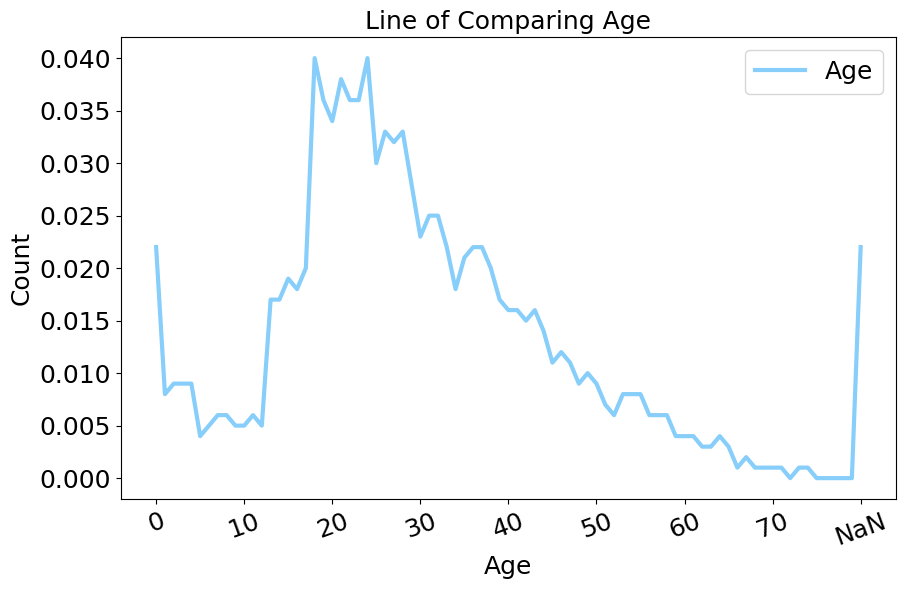
\includegraphics[scale=0.35]{Sec2_15.png}
            }
            \subfigure[Age与Transported]
            {
                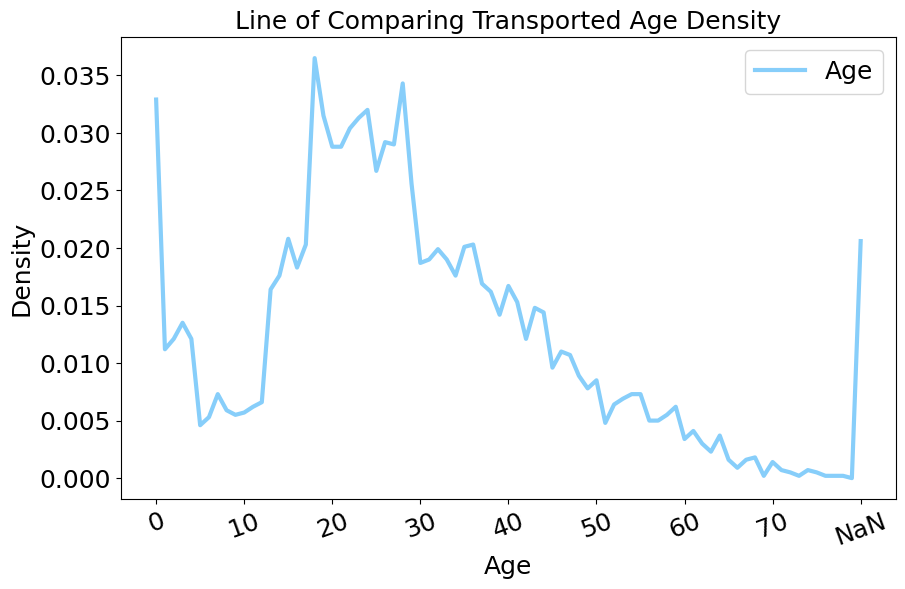
\includegraphics[scale=0.35]{Sec2_16.png}
            }
            \caption{Age}
        \end{figure}

        查看Expenditure与Transported之间的关系,其中RoomService,FoodCourt,ShoppingMall,Spa,VRDeck分别如图10,11,12,13,14所示。
        可以发现无论是哪种消费,都主要集中在少于5000的位置,并且RoomService和FoodCourt更贴近日常人们的生活需求,因此消费人群较多。
        但是查看不同消费树木中被传送的人群密度图,可以发现整个曲线呈现一个突变的状态,一方面是因为这里面不同数值太多,并没有提前进行分组,另一方面也是因为除了RoomService外的消费特征与Transported的相关性都并不强。
        RoomService指的是住房需求,在前面的分析中我们可以得出没有休眠的人更容易被传送走,而RoomService消费越少就代表乘客休息的次数应该也是越少的,而从密度图中可以看出,RoomService消费越少的人群中被传送的比例相比起来远远高于RoomService消费高的人群。
        
        \begin{figure}[H]
            \centering
            \subfigure[RoomService对比]
            {
                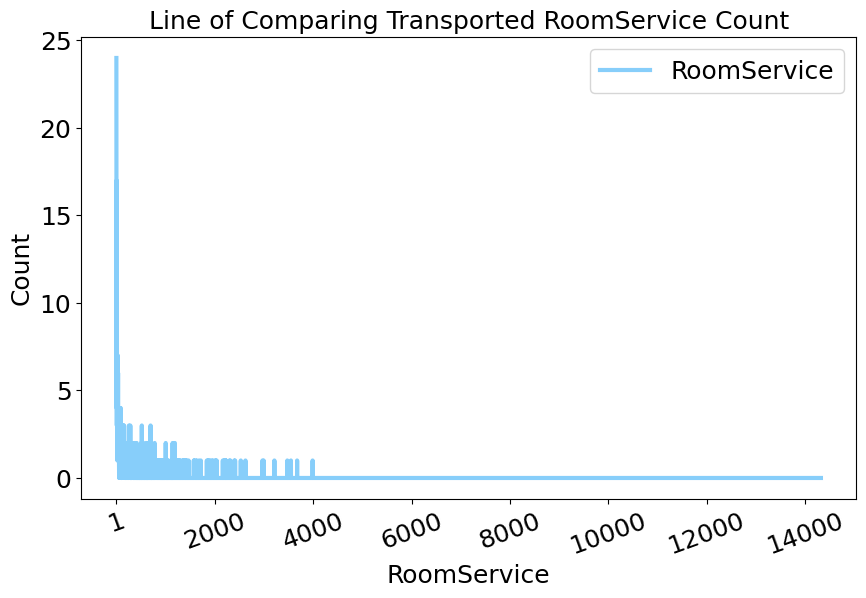
\includegraphics[scale=0.25]{Sec2_17.png}
            }
            \subfigure[RoomService与Transported]
            {
                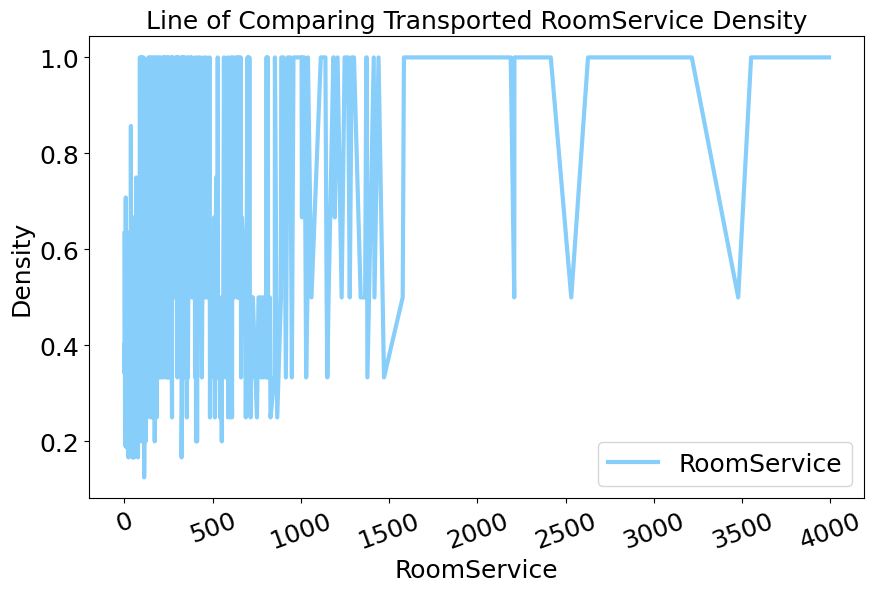
\includegraphics[scale=0.25]{Sec2_18.png}
            }
            \caption{RoomService}
        \end{figure}

        \begin{figure}[H]
            \centering
            \subfigure[FoodCourt对比]
            {
                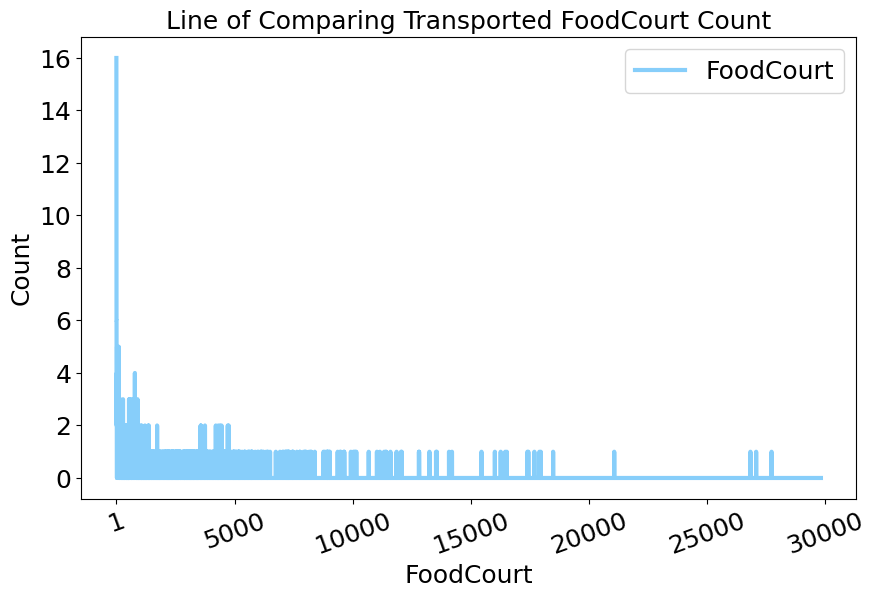
\includegraphics[scale=0.25]{Sec2_19.png}
            }
            \subfigure[FoodCourt与Transported]
            {
                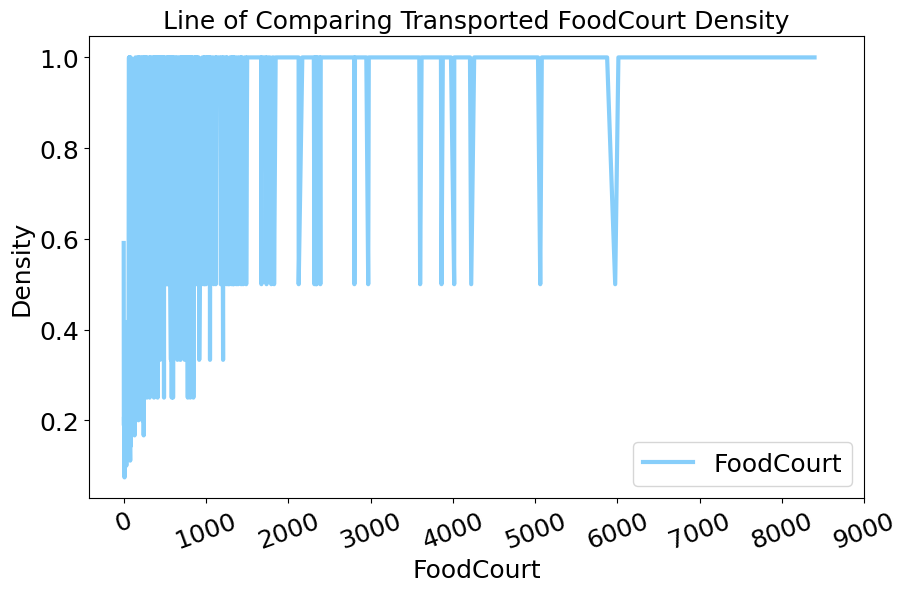
\includegraphics[scale=0.25]{Sec2_20.png}
            }
            \caption{FoodCourt}
        \end{figure}

        \begin{figure}[H]
            \centering
            \subfigure[ShoppingMall对比]
            {
                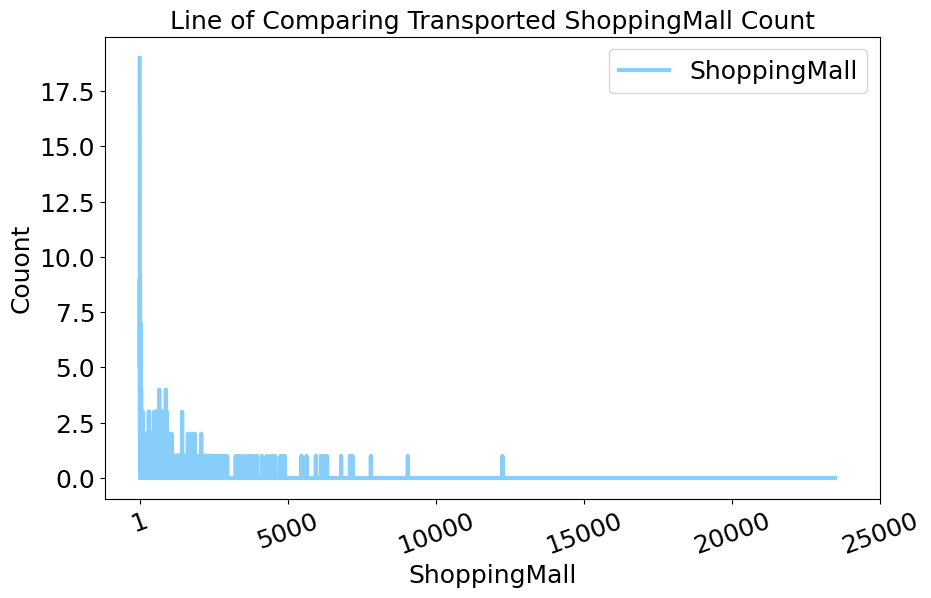
\includegraphics[scale=0.25]{Sec2_21.png}
            }
            \subfigure[ShoppingMall与Transported]
            {
                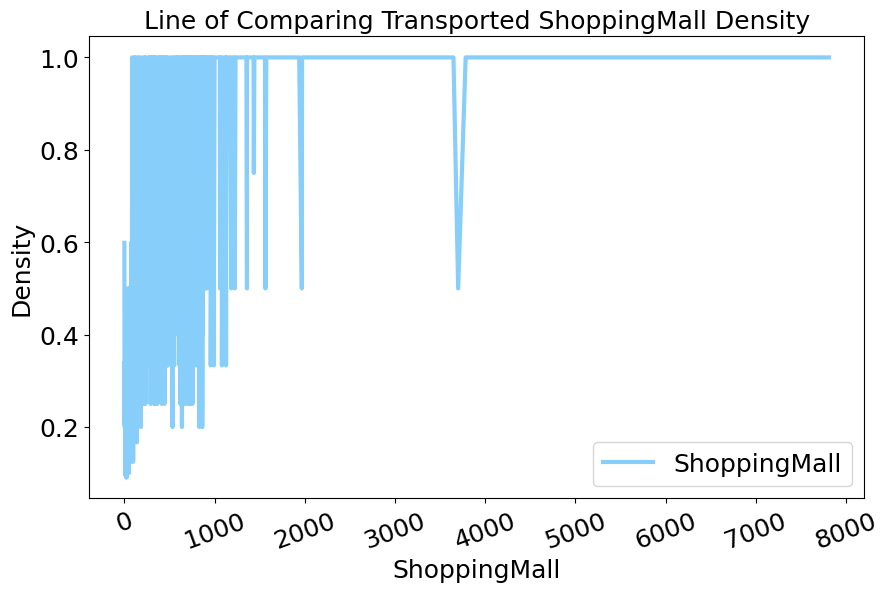
\includegraphics[scale=0.25]{Sec2_22.png}
            }
            \caption{ShoppingMall}
        \end{figure}

        \begin{figure}[H]
            \centering
            \subfigure[Spa对比]
            {
                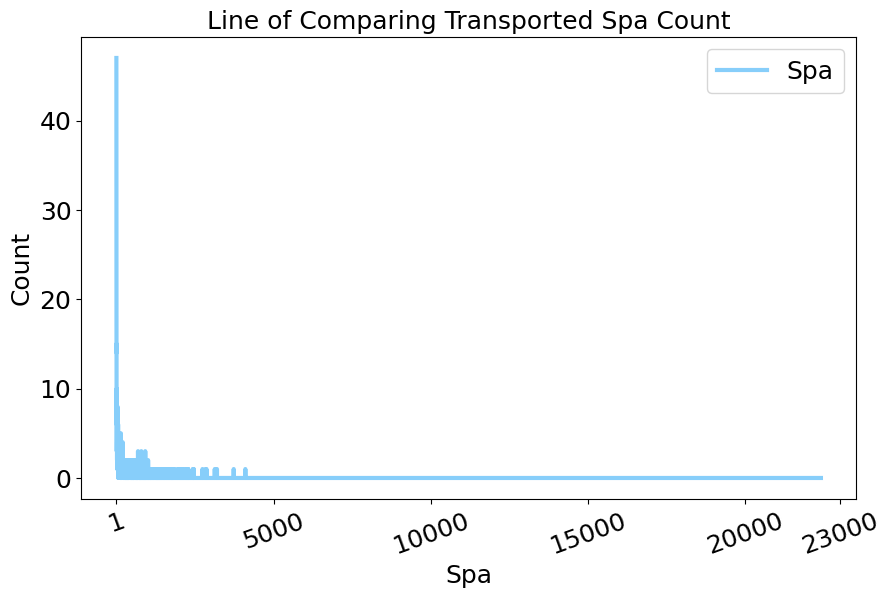
\includegraphics[scale=0.25]{Sec2_23.png}
            }
            \subfigure[Spa与Transported]
            {
                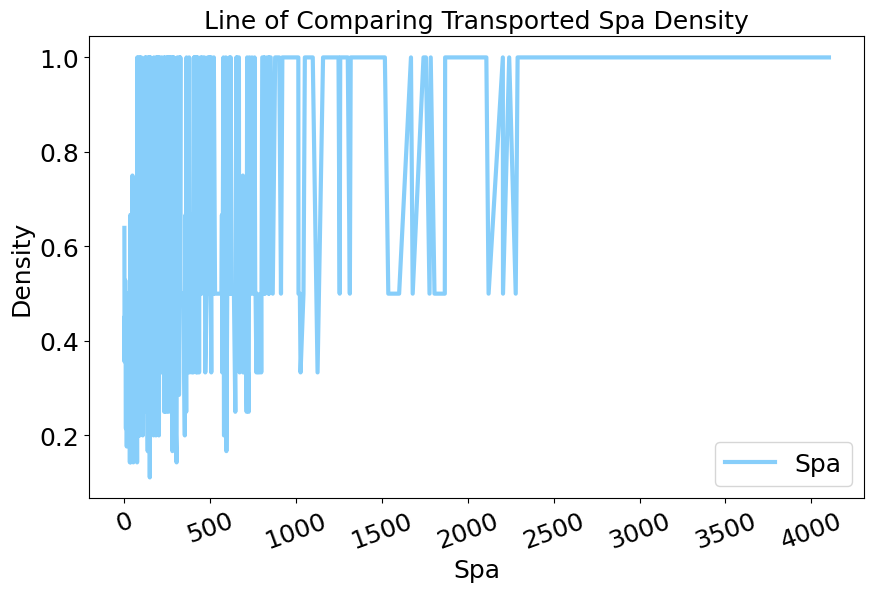
\includegraphics[scale=0.25]{Sec2_24.png}
            }
            \caption{Spa}
        \end{figure}

        \begin{figure}[H]
            \centering
            \subfigure[VRDeck对比]
            {
                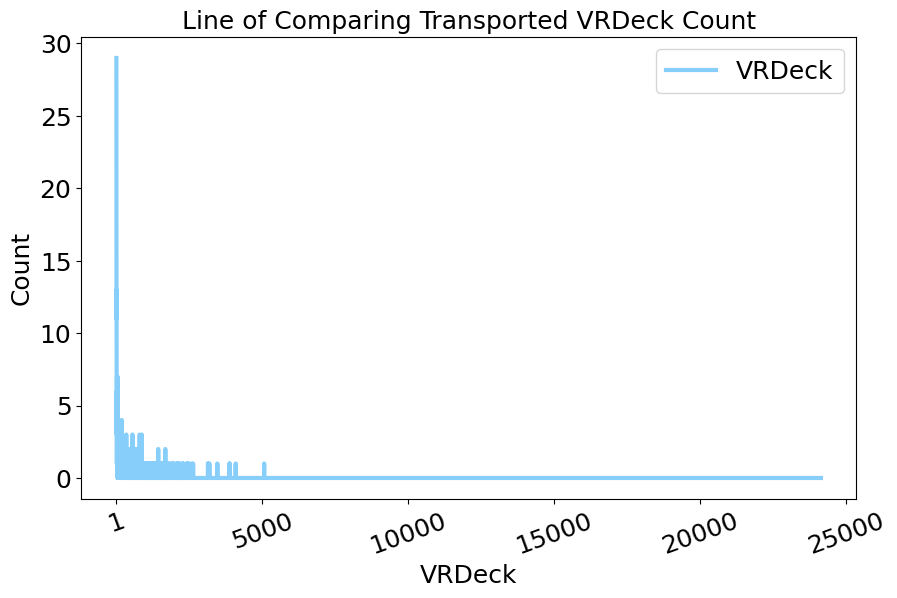
\includegraphics[scale=0.25]{Sec2_25.png}
            }
            \subfigure[VRDeck与Transported]
            {
                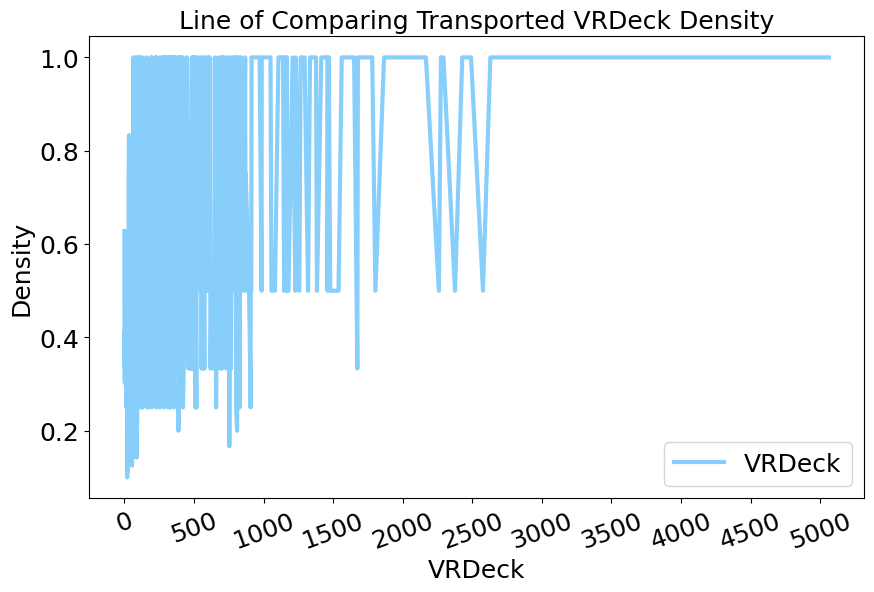
\includegraphics[scale=0.25]{Sec2_26.png}
            }
            \caption{VRDeck}
        \end{figure}

        查看PassengerId与Transported之间的关系,如图15所示。
        由于PassengerId的格式问题,前面的pppp可以被称为Group,而后面的gg是一个较为随机的数字,因此主要分析的应该是Group与Transported之间的关系。
        而如果直接查看不同Group之中的人数,得到的图可以发现大多数Group的人数主要集中在1-3个人,较少超过4个人。
        因此我们可以得到一个Group\_Size的特征,即所在的Group有多少人,并查看不同Group\_Size中被传送与不被传送的关系,可以发现的是只有Group\_Size为1的时候被传送的人数少于不被传送的乘客数。
        所以我还新加入了一个特征Alone来记录该乘客是否为自己一人旅行,这个时候他被传送的概率应该较高。

        \begin{figure}[H]
            \centering
            \subfigure[Group对比]
            {
                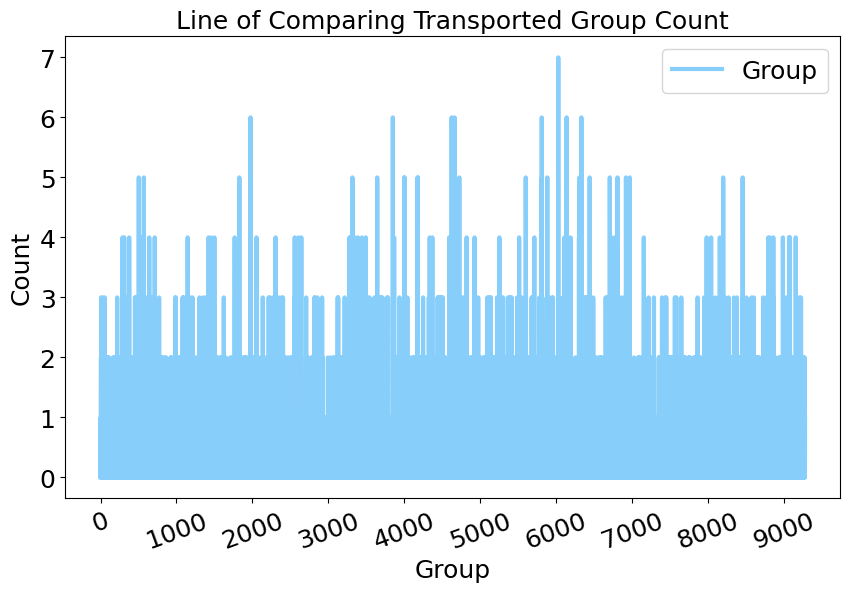
\includegraphics[scale=0.3]{Sec2_27.png}
            }
            \subfigure[Group\_Size与Transported]
            {
                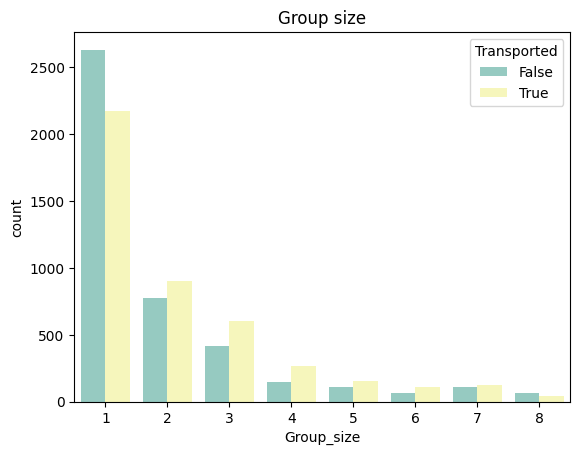
\includegraphics[scale=0.3]{Sec2_28.png}
            }
            \caption{PassengerId}
        \end{figure}

        查看Cabin与Transported之间的关系,如图16所示。
        由于Cabin的格式问题,有三个数据Deck/Number/Side,因此将其拆分成为三个数据Cabin\_Deck,Cabin\_Number,Cabin\_Side进行分析。
        可以发现Cabin\_Deck中乘客的人数集中在F和G,然而被传送比例最高的反而是B和C,并且结合之前的信息我们可以发现Cabin\_Deck,HomePlanet和Destination特征的取值主要集中在几个变量上,因此我决定后续对于Cabin\_Deck及这三个特征的关系进行更深入的探究。
        而Cabin\_Number和PassengerId一样,较为分散,难以看出什么分布,所以不做更多分析(这张图我不知道画的时候有什么问题,显示不出颜色)。
        最后查看Cabin\_Side,由于他只有两种取值,P或S,因此直接查看可以发现Side为P的乘客被传送的几率较小,而为S的乘客被传送的几率较大,但是两者相差不大,因此后续对于Cabin\_Side的关注度并不高。

        \begin{figure}[H]
            \centering
            \subfigure[Cabin\_Deck对比]
            {
                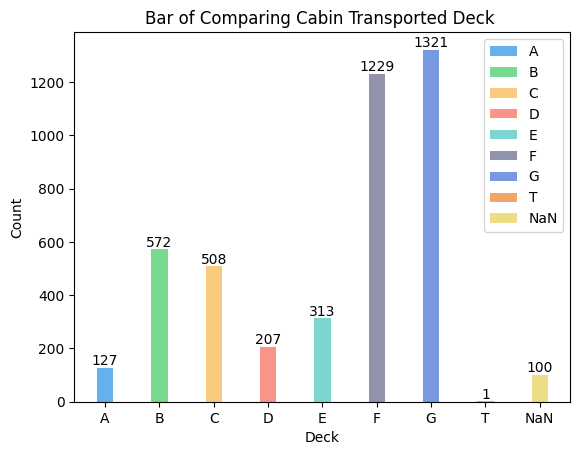
\includegraphics[scale=0.3]{Sec2_29.png}
            }
            \subfigure[Cabin\_Deck与Transported]
            {
                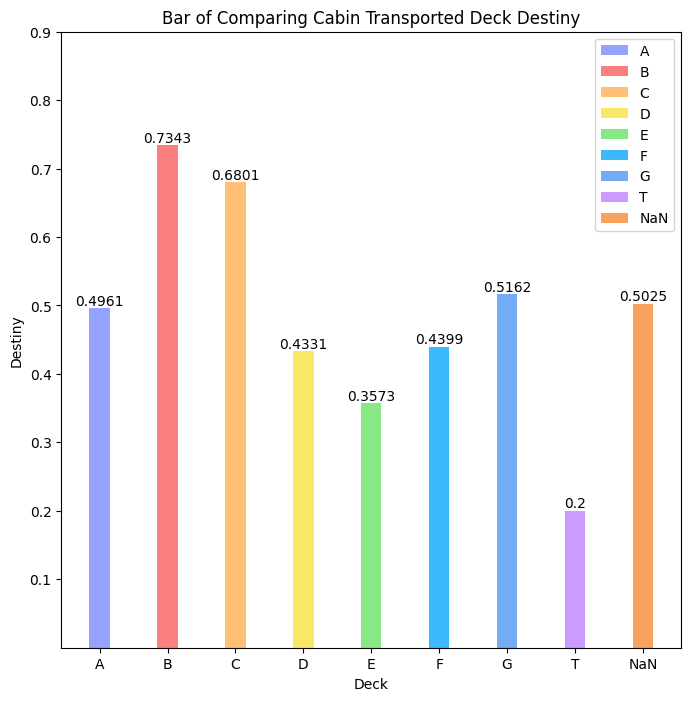
\includegraphics[scale=0.3]{Sec2_30.png}
            }
            
            \subfigure[Cabin\_Number]
            {
                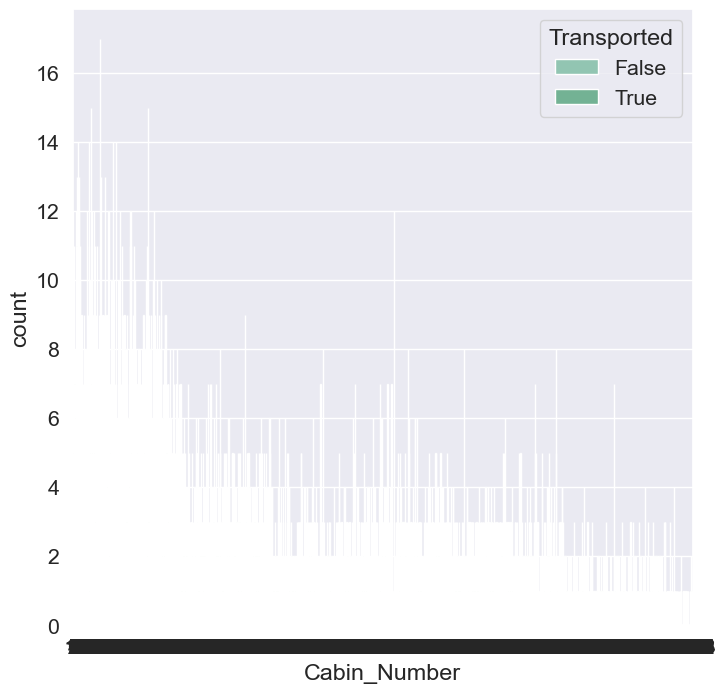
\includegraphics[scale=0.3]{Sec2_31.png}
            }
            \subfigure[Cabin\_Side]
            {
                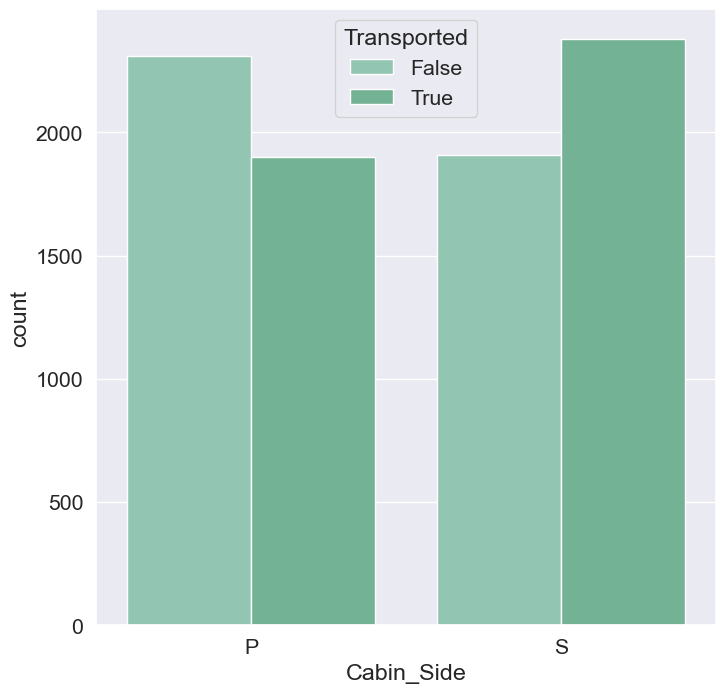
\includegraphics[scale=0.3]{Sec2_32.png}
            }
            \caption{Cabin}
        \end{figure}

\end{document}